\documentclass[12pt, titlepage]{article}

\usepackage{booktabs}
\usepackage{tabularx}
\usepackage{hyperref}
\usepackage{graphicx}
\usepackage{amsmath, mathtools}
\usepackage{amsfonts}
\usepackage{amssymb}
\usepackage{graphicx}
\usepackage{colortbl}
\usepackage{xr}
\usepackage{hyperref}
\usepackage{longtable}
\usepackage{xfrac}
\usepackage{tabularx}
\usepackage{float}
\usepackage{siunitx}
\usepackage{booktabs}
\usepackage{caption}
\usepackage{pdflscape}
\usepackage{afterpage}
\hypersetup{
    colorlinks,
    citecolor=black,
    filecolor=black,
    linkcolor=red,
    urlcolor=blue
}
\usepackage[round]{natbib}

%% Comments

\usepackage{color}

\newif\ifcomments\commentstrue

\ifcomments
\newcommand{\authornote}[3]{\textcolor{#1}{[#3 ---#2]}}
\newcommand{\todo}[1]{\textcolor{red}{[TODO: #1]}}
\else
\newcommand{\authornote}[3]{}
\newcommand{\todo}[1]{}
\fi

\newcommand{\wss}[1]{\authornote{blue}{SS}{#1}}
\newcommand{\an}[1]{\authornote{magenta}{Author}{#1}}
\newcommand{\wss}[1]{\authornote{blue}{SS}{#1}}



\begin{document}

\title{FFT Library} 
\author{Yuzhi Zhao}
\date{\today}
	
\maketitle

\pagenumbering{roman}

\section{Revision History}

\begin{tabularx}{\textwidth}{p{3cm}p{2cm}X}
\toprule {\bf Date} & {\bf Version} & {\bf Notes}\\
\midrule
Date 1 & 1.0 & Notes\\
Date 2 & 1.1 & Notes\\
\bottomrule
\end{tabularx}

~\newpage

\section{Symbols, Abbreviations and Acronyms}

\renewcommand{\arraystretch}{1.2}
\begin{tabular}{l l} 
  \toprule		
  \textbf{symbol} & \textbf{description}\\
  \midrule 
  T & Test\\
  \bottomrule
\end{tabular}\\

\newpage

\tableofcontents

\listoftables

\listoffigures

\newpage

\pagenumbering{arabic}


\section{General Information}
The following section provides an overview of the Verification and Validation (V \& V) Plan for a FFT library.

\subsection{Purpose}
The main purpose of this document is to describe the verification and validation process
that will be used to test a FFT Library.This document is intended to be used as a reference for all future testing and will be used
to increase confidence in the software implementation.\\
This document will be used as a starting point for the verification and validation report.
The test cases presented within this document will be executed and the output will be
analyzed to determine if the library is implemented correctly.

\subsection{Scope}
The whole library includes four FFT or IFFT calculation functions. All tests should be applied based on this scope.

\subsection{Overview of Document}
The following sections provides more details about the V\&V of a FFT Library. Information about verification tools, automated testing approaches will be stated. And
test cases for all system testing and part of unit testing will be provided.
\section{Plan}
	
\subsection{Software Description}
The software being tested is a library for FFT algorithm. Users choose different  FFT or IFFT functions and give proper input datas to complete a FFT or IFFT calculation. 
The library includes radix-2 and radix-3 FFT(and IFFT) calculation functions.
\subsection{Test Team}
Yuzhi Zhao

\subsection{Automated Testing Approach}
A unit testing framework will be implemented in both unit testing and system testing.\\
Script will be used to call all the test cases in test suite.\\
Test coverage analysis will be applied to measure code coverage.\\
Compiler can do syntax check automatically.

\subsection{Verification Tools}
\begin{enumerate}
\item {{\large Cutest} as unit testing framework}
\item {{\large Make} as script to call test cases and execute test}
\item {{\large Xcover} as coverage analysis tool}
\end{enumerate}

% \subsection{Testing Schedule}
		
% See Gantt Chart at the following url ...

\subsection{Non-Testing Based Verification}
{\large Symbolic Execution}

Because FFT library is based on a mathematical expression. Using Symbolic Execution can trace the path and the result can be compared with mathematical expression directly.



\section{System Test Description}
	
\subsection{Tests for Functional Requirements}

\subsubsection{Calculation Test}
		
\paragraph{Radix-2 Complex Number Calculation Function\\}

\begin{enumerate}

\item{Radix-2 Complex Number FFT Calculation Function\\}

\textbf {Type}: Functional, Dynamic, Automated
					
\textbf {Initial State}: None
					
\textbf {Input}:\\ input.txt :  Includes all the input datas. Two exmples of input.txt is shown in Figure~\ref{Fig_Inputcomplex} and Figure~\ref{Fig_Inputfloating}.\\ 
 expectedOutput.txt:  Includes the output datas using the same input datas but computed by Matlab FFT library. Then output.txts  are shown in Figure~\ref{Fig_Inputcomplex} and Figure~\ref{Fig_Inputfloating}. \\ 
If the numbers of data can not satisfy $2^n$, program will automatically fill with 0.\\
					
\textbf {Output}:  output.txt : Includes the output datas using the input data computed by this FFT library.\\
TestResult: pass or not pass. Whether the program passed the test is measured by an admissible error and the algorithm for the admissible erro is provided as below:\\



\begin{figure}[h!]
\centering
\begin{minipage}[b]{0.4\textwidth}
 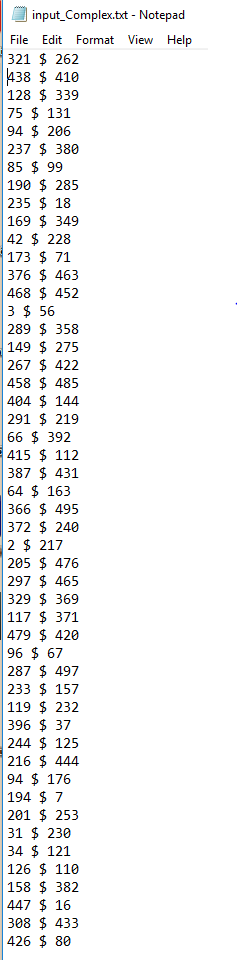
\includegraphics[width=\textwidth]{Input_complex}
\caption{System Context}
\label{Fig_Inputcomplex} 
\end{minipage}
\hfill
\begin{minipage}[b]{0.31\textwidth}
 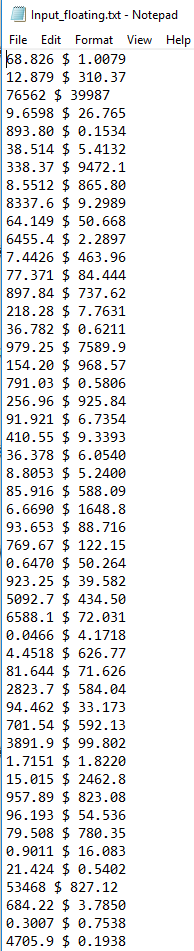
\includegraphics[width=\textwidth]{Input_floating}
\caption{System Context}
\label{Fig_Inputfloating} 
\end{minipage}
\end{figure}
		
\begin{figure}[h!]
\centering
\begin{minipage}[b]{0.4\textwidth}
 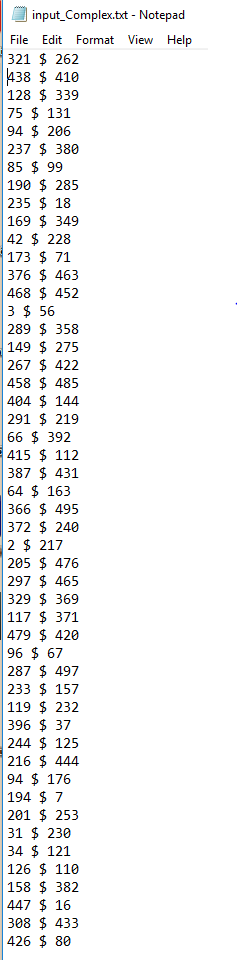
\includegraphics[width=\textwidth]{Input_complex}
\caption{System Context}
\label{Fig_Inputcomplex} 
\end{minipage}
\hfill
\begin{minipage}[b]{0.31\textwidth}
 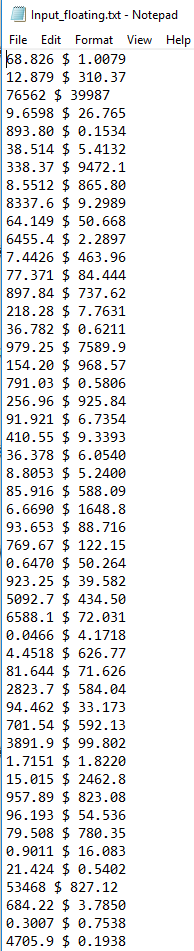
\includegraphics[width=\textwidth]{Input_floating}
\caption{System Context}
\label{Fig_Inputfloating} 
\end{minipage}
\end{figure}
			
\textbf {How test will be performed}: \\
Automated.
For validation purpose, datas should also be compared with results from normal DFT calculations manually.

\item{Radix-2 Complex Number IFFT Calculation Function\\}

\textbf {Type}: Functional, Dynamic, Automated
					
\textbf {Initial State}: None
					
\textbf {Input}: input.txt, expectedOutput.txt
					
\textbf {Output}:  output.txt, TestResult: pass or not pass

\textbf {How test will be performed}: \\
Same as above.
\end{enumerate}

					
\paragraph{Radix-2 Real Number Calculation Function\\}

\begin{enumerate}

\item{Radix-2 Real Number FFT Calculation Function\\}

\textbf {Type}: Functional, Dynamic, Automated
					
\textbf {Initial State}: None
					
\textbf {Input}: input.txt, expectedOutput.txt
					
\textbf {Output}:  output.txt, TestResult: pass or not pass
					
\textbf {How test will be performed}: \\
Same as above.

\item{Radix-2 Real Number IFFT Calculation Function\\}

\textbf {Type}: Functional, Dynamic, Automated
					
\textbf {Initial State}: None
					
\textbf {Input}: input.txt, expectedOutput.txt
					
\textbf {Output}:  output.txt, TestResult: pass or not pass

\textbf {How test will be performed}: \\
Same as above.
\end{enumerate}

\paragraph{Radix-3 Complex Number Calculation Function\\}

\begin{enumerate}

\item{Radix-3 Complex Number FFT Calculation Function\\}

\textbf {Type}: Functional, Dynamic, Automated

\textbf {Initial State}: None
					
\textbf {Input}: input.txt, expectedOutput.txt
					
\textbf {Output}:  output.txt, TestResult: pass or not pass
					
\textbf {How test will be performed}: \\
Same as above.

\item{Radix-3 Complex Number IFFT Calculation Function\\}

\textbf {Type}: Functional, Dynamic, Automated
					
\textbf {Initial State}: None
					
\textbf {Input}: input.txt, expectedOutput.txt
					
\textbf {Output}:  output.txt, TestResult: pass or not pass

\textbf {How test will be performed}: \\
Same as above.
\end{enumerate}

\paragraph{Radix-3 Real Number Calculation Function\\}

\begin{enumerate}

\item{Radix-3 Real Number FFT Calculation Function\\}

\textbf {Type}: Functional, Dynamic, Automated
					
\textbf {Initial State}: None
					
\textbf {Input}: input.txt, expectedOutput.txt
					
\textbf {Output}:  output.txt, TestResult: pass or not pass
					
\textbf {How test will be performed}: \\


\item{Radix-3 Real Number IFFT Calculation Function\\}

\textbf {Type}: Functional, Dynamic, Automated
					
\textbf {Initial State}: None
					
\textbf {Input}: input.txt, expectedOutput.txt
					
\textbf {Output}:  output.txt, TestResult: pass or not pass

\textbf {How test will be performed}: \\
Same as above.
\end{enumerate}

\subsubsection{Loading Library Test}

\paragraph{Under Win X86 plateform\\}

\textbf {Type}: Functional, Dynamic, Manual
					
\textbf {Initial State}: None
					
\textbf {Input}: input.txt
					
\textbf {Output}: output.txt
					
\textbf {How test will be performed}: Manual, automated


\paragraph{Under Mac OS plateform\\}

\textbf {Type}: Functional, Dynamic, Manual
					
\textbf {Initial State}: None
					
\textbf {Input}: input.txt
					
\textbf {Output}: output.txt
					
\textbf {How test will be performed}: Manual,automated



\subsection{Tests for Nonfunctional Requirements}

\subsubsection{Speed Comparation Test}
		
\paragraph{Compare Calculation Speed with DFT calculation\\}

\textbf {Type}: Dynamic, automated, Manual
					
\textbf {Initial State}: None
					
\textbf {Input}: intput.txt
					
\textbf {Output}: Time
					
\textbf {How test will be performed}: \\
Manually compare the time with the time using DFT Library.


\subsection{Traceability Between Test Cases and Requirements}

% \section{Tests for Proof of Concept}

% \subsection{Area of Testing1}
		
% \paragraph{Title for Test}

% \begin{enumerate}

% \item{test-id1\\}

% Type: Functional, Dynamic, Manual, Static etc.
					
% Initial State: 
					
% Input: 
					
% Output: 
					
% How test will be performed: 
					
% \item{test-id2\\}

% Type: Functional, Dynamic, Manual, Static etc.
					
% Initial State: 
					
% Input: 
					
% Output: 
					
% How test will be performed: 

% \end{enumerate}

% \subsection{Area of Testing2}

% ...
				
\section{Unit Testing Plan}
		
\wss{Unit testing plans for internal functions and, if appropriate, output
  files}

\bibliographystyle{plainnat}

\bibliography{SRS}

\newpage

\section{Appendix}

This is where you can place additional information.

\subsection{Symbolic Parameters}

The definition of the test cases will call for SYMBOLIC\_CONSTANTS.
Their values are defined in this section for easy maintenance.

\subsection{Usability Survey Questions?}

This is a section that would be appropriate for some teams.

\end{document}